\documentclass[12pt]{article}
\linespread{1.3}
\usepackage{hyperref}
\usepackage{enumitem}
%\usepackage{enumerate}
\usepackage{changepage,lipsum,titlesec, longtable}
\usepackage{cite}
\usepackage{comment, xcolor}
\usepackage[pdftex]{graphicx}
  \graphicspath{{images/}, {images/stat/}}
  \DeclareGraphicsExtensions{.pdf,.jpeg,.png, .jpg}
\usepackage[cmex10]{amsmath}
\usepackage{tikz}
\usepackage{array} 
\usepackage{subfigure} 
\newcommand{\grey}[1]{\textcolor{black!30}{#1}}
\newcommand{\red}[1]{\textcolor{red!50}{#1}}
\newcommand{\fref}[1]{Figure~\ref{#1}}
\newcommand{\tref}[1]{Table~\ref{#1}}
\newcommand{\eref}[1]{Equation~\ref{#1}}
\newcommand{\cref}[1]{Chapter~\ref{#1}}
\newcommand{\sref}[1]{Section~\ref{#1}}
\newcommand{\aref}[1]{Appendix~\ref{#1}}

\renewcommand{\labelenumii}{\theenumii}
\renewcommand{\theenumii}{\theenumi.\\arabic{enumii}.}

\oddsidemargin0cm
\topmargin-2cm %I recommend adding these three lines to increase the
\textwidth16.5cm %amount of usable space on the page (and save trees)
\textheight23.5cm

\makeatletter
\renewcommand\paragraph{\@startsection{paragraph}{4}{\z@}%
            {-2.5ex\@plus -1ex \@minus -.25ex}%
            {1.25ex \@plus .25ex}%
            {\normalfont\normalsize\bfseries}}
\makeatother
\setcounter{secnumdepth}{4} % how many sectioning levels to assign numbers to
\setcounter{tocdepth}{4}    % how many sectioning levels to show in ToC


\begin{document}
\title{PM table to json converter\\
       \large SEED project}
\maketitle
\tableofcontents
\newpage
\section{Matching and mapping SEED and PM}\label{sec:map}

  The following description of the connection between Portfolio
  Manager and SEED platform is summarized from ~\cite{SEEDTutorial2015}

  For commercial building benchmarking, the city government need to
  acquire energy consumption data of buildings in the city. As a
  result, there are requirements to collect building energy
  consumption information for buildings greater than 5000 sq. ft. The
  city will create a list of buildings they need to collect energy
  information from. The owners of the buildings in the list will
  report the energy consumption data through the
  \href{https://portfoliomanager.energystar.gov/pm/home.html}{Portfolio
    Manager} developed by U.S. Environmental Protection Agency
  (EPA)and share the report with the city. The city can government can
  download the data from the Portfolio Manager site into one big
  folder. 
  
  \fref{fig:seedDiagram} is the diagram of the SEED platform
  \begin{figure}[h!]
    \centering
    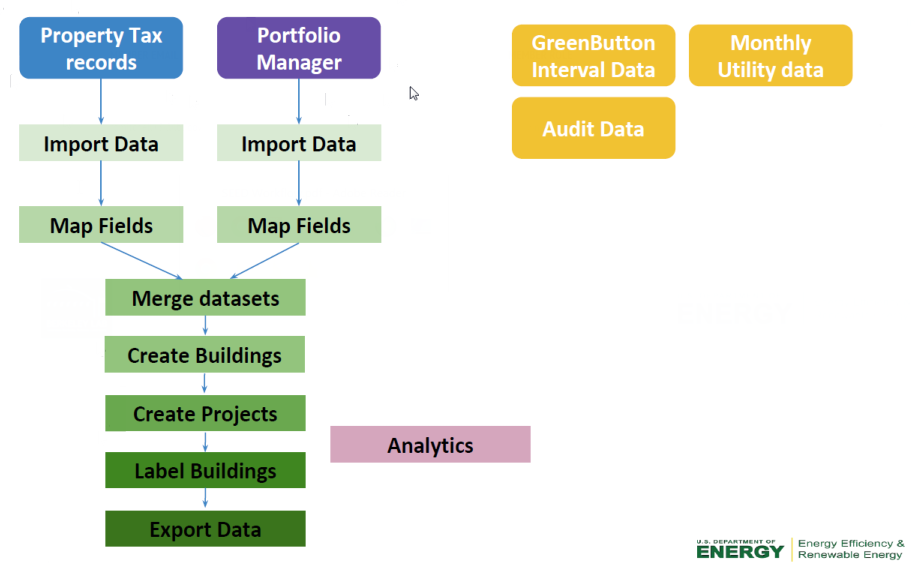
\includegraphics[width = 0.7\textwidth]{seedDiagram.png}
    \caption{SEED flow diagram}~\cite{SEEDTutorial2015}
    \label{fig:seedDiagram}
  \end{figure}

  In order to hold and process the large amount of data, a database is
  needed. DOE developed the SEED platform to assist cities to manage
  the building energy consumption data. The city government would
  import 1) the list of buildings into the SEED database, and 2)
  import the energy consumption data from the portfolio manager. 

  The two sets of data just imported would go through a process called
  \textbf{``Map Fields'' (Mapping)} which standardized the fields of
  the two data sources. Then \textbf{``Matching''} (using fuzzy logic)
  is performed between the two so that the building is associated with
  its energy consumption records. Then the database is ready to carry
  out analysis.
  
  In the ``Mapping'' process, the program will predict based on the
  original name of the excel sheet user uploaded (my understanding)
  and the user will confirm which field of the original uploaded data
  is associated to the standard database field.
  
  Other sources of data started to be incorporated into the SEED
  platform: GreenButton Data (short interval energy consumption data )
  and Audit Data
  (\href{https://www.ashrae.org/resources--publications/bookstore/procedures-for-commercial-building-energy-audits}{Procedures
    For Commercial Building Energy Audits}).

  Building list: the fields in the building list include: UBI(?),
  GBA(Gross Building Area), BLDGS, Address, Owner, City, State, Zip,
  Property Type, AYB\_YearBuilt. PM data has fields such as: Property
  ID, Property Name, YearEnding, PropertyFloorArea, Address 1, Address
  2, City, ... Although the two might both have ID field, they might
  not be related. The suggested field for matching the building list
  with the PM data is with Address (``Address Line 1'' in SEED). In
  general, there are four suggested fields that \textbf{improve the
    matching result: Tax Lot ID, PM Property ID (``Property ID'' field
    in PM), Custom ID and Address Line 1}(\fref{fig:matching}).
  
  \begin{figure}[h!]
    \centering
    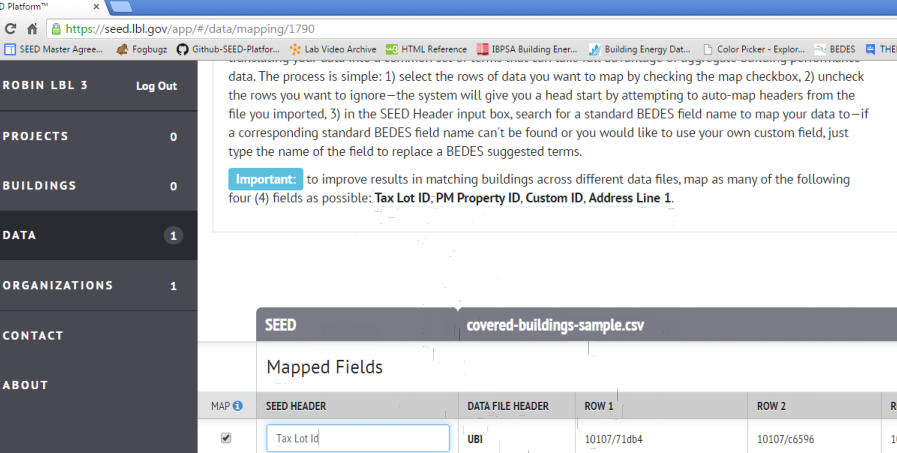
\includegraphics[width = 1.0\textwidth]{matching.png}
    \caption{Matching requirement}~\cite{SEEDTutorial2015}
    \label{fig:matching}
  \end{figure}
\section{Template Development}
Based on the suggested field for improving data matching performance,
the following template is created (\fref{fig:template}):

\begin{figure}[h!]
  \centering
  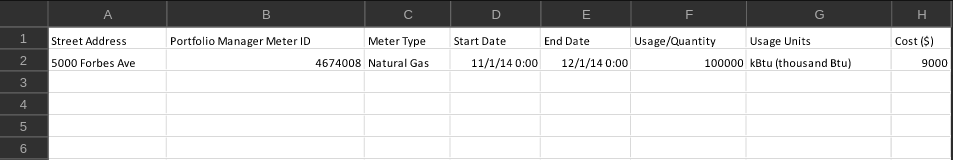
\includegraphics[width = 1.0\textwidth]{template.png}
  \caption{Excel template}
  \label{fig:template}
\end{figure}

\pagebreak
\section{Code}
\makeatletter
\def\verbatim@font{\linespread{1}\tiny\ttfamily}
\makeatother
\begin{verbatim}
## ## ## ## ## ## ## ## ## ## ## ## ## ## ## 
## converter.py
## ## ## ## ## ## ## ## ## ## ## ## ## ## ## 
import os 
import pandas as pd
import json

# replace the following directory name and filename
read_dir_name = os.getcwd() + "/PMfile/"
read_file_name = "template.xlsx"
read_sheet_name = 0
write_dir_name = os.getcwd() + "/Jsonfile/"
write_file_name = "test.txt"

def pm2json():
    meter_con_df = pd.read_excel(read_dir_name + read_file_name,
                                 sheetname=read_sheet_name, skiprows=0,
                                 header = 0)

    # Calculate time interval of days
    meter_con_df['interval'] = meter_con_df['End Date'] - meter_con_df['Start Date']
    meter_con_df['reading_kind'] = 'energy'

    # renaming columns of df
    name_lookup = {u'Start Date':u'start',
                   u'End Date':u'end',
                   u'Portfolio Manager Meter ID':u'meter_id',
                   u'Usage/Quantity':u'value',
                   u'Usage Units':'uom'}

    meter_con_df = meter_con_df.rename(columns=name_lookup)

    # the 'interval' output is in [ns], so use ns for all time object and
    # post process with postProcess.py
    meter_con_df.to_json(write_dir_name + write_file_name, 'records',
                         date_unit = 'ns')

## ## ## ## ## ## ## ## ## ## ## ## ## ## ## 
## postProcess.py
## ## ## ## ## ## ## ## ## ## ## ## ## ## ## 
import os 
import converter as cv

dir_name = os.getcwd() + "/Jsonfile/"
in_file_name = cv.write_file_name
out_file_name = "post_test.txt"

# convert unit of time from 'ns' to 's'
def ns2s(string):
    return string.replace('000000000,', ',')

def postProcess():
    with open (dir_name + in_file_name, 'r+') as infile:
        unit_ns = infile.readline()
        unit_s = ns2s(unit_ns)
    with open (dir_name + out_file_name, 'w') as out:
        out.write(unit_s)

## ## ## ## ## ## ## ## ## ## ## ## ## ## ## 
## mainroutine.py
## ## ## ## ## ## ## ## ## ## ## ## ## ## ## 
import converter as cv 
import postProcess as ps

cv.pm2json()
ps.postProcess()

\end{verbatim}
\section{Output} 

\begin{verbatim}
[{"Street Address":"5000 Forbes Ave","meter_id":4674008,"Meter Type":"Natural Gas","start":1414800000,
"end":1417392000,"value":100000,"uom":"kBtu (thousand Btu)","Cost ($)":9000,"interval":2592000,"reading_kind":"energy"}] 
\end{verbatim}
\newpage
\bibliographystyle{plain}
\bibliography{myCitation}
\end{document}